\newpage
\section{Model}
\label{sec:model}

In this section, we present our model of the energy procurement problem for geo-distributed data centers participating in multi-timescale markets. For analytical tractability, we consider a two-timescale setting, consisting of a long-term electricity market and a real-time electricity market.

\subsection{System model}

\desc{System model}

%\todo{Should we consider adding forward market (intermididate) as well. This is very challenging as the objective function can be non-convex because of the GLB components. It cannot be solved in this version.}

\textbf{Two-timescale markets}. A service provider operating geo-distributed data centers can purchase electricity in two markets -- a long-term market and a real-time market. The electricity consumed at time $t=0$ must be procured from the real-time market at $t=0$ and/or from the long term market {\em ahead of time} at $t=-T_l$. 

\begin{figure}[!t]
	\centering
	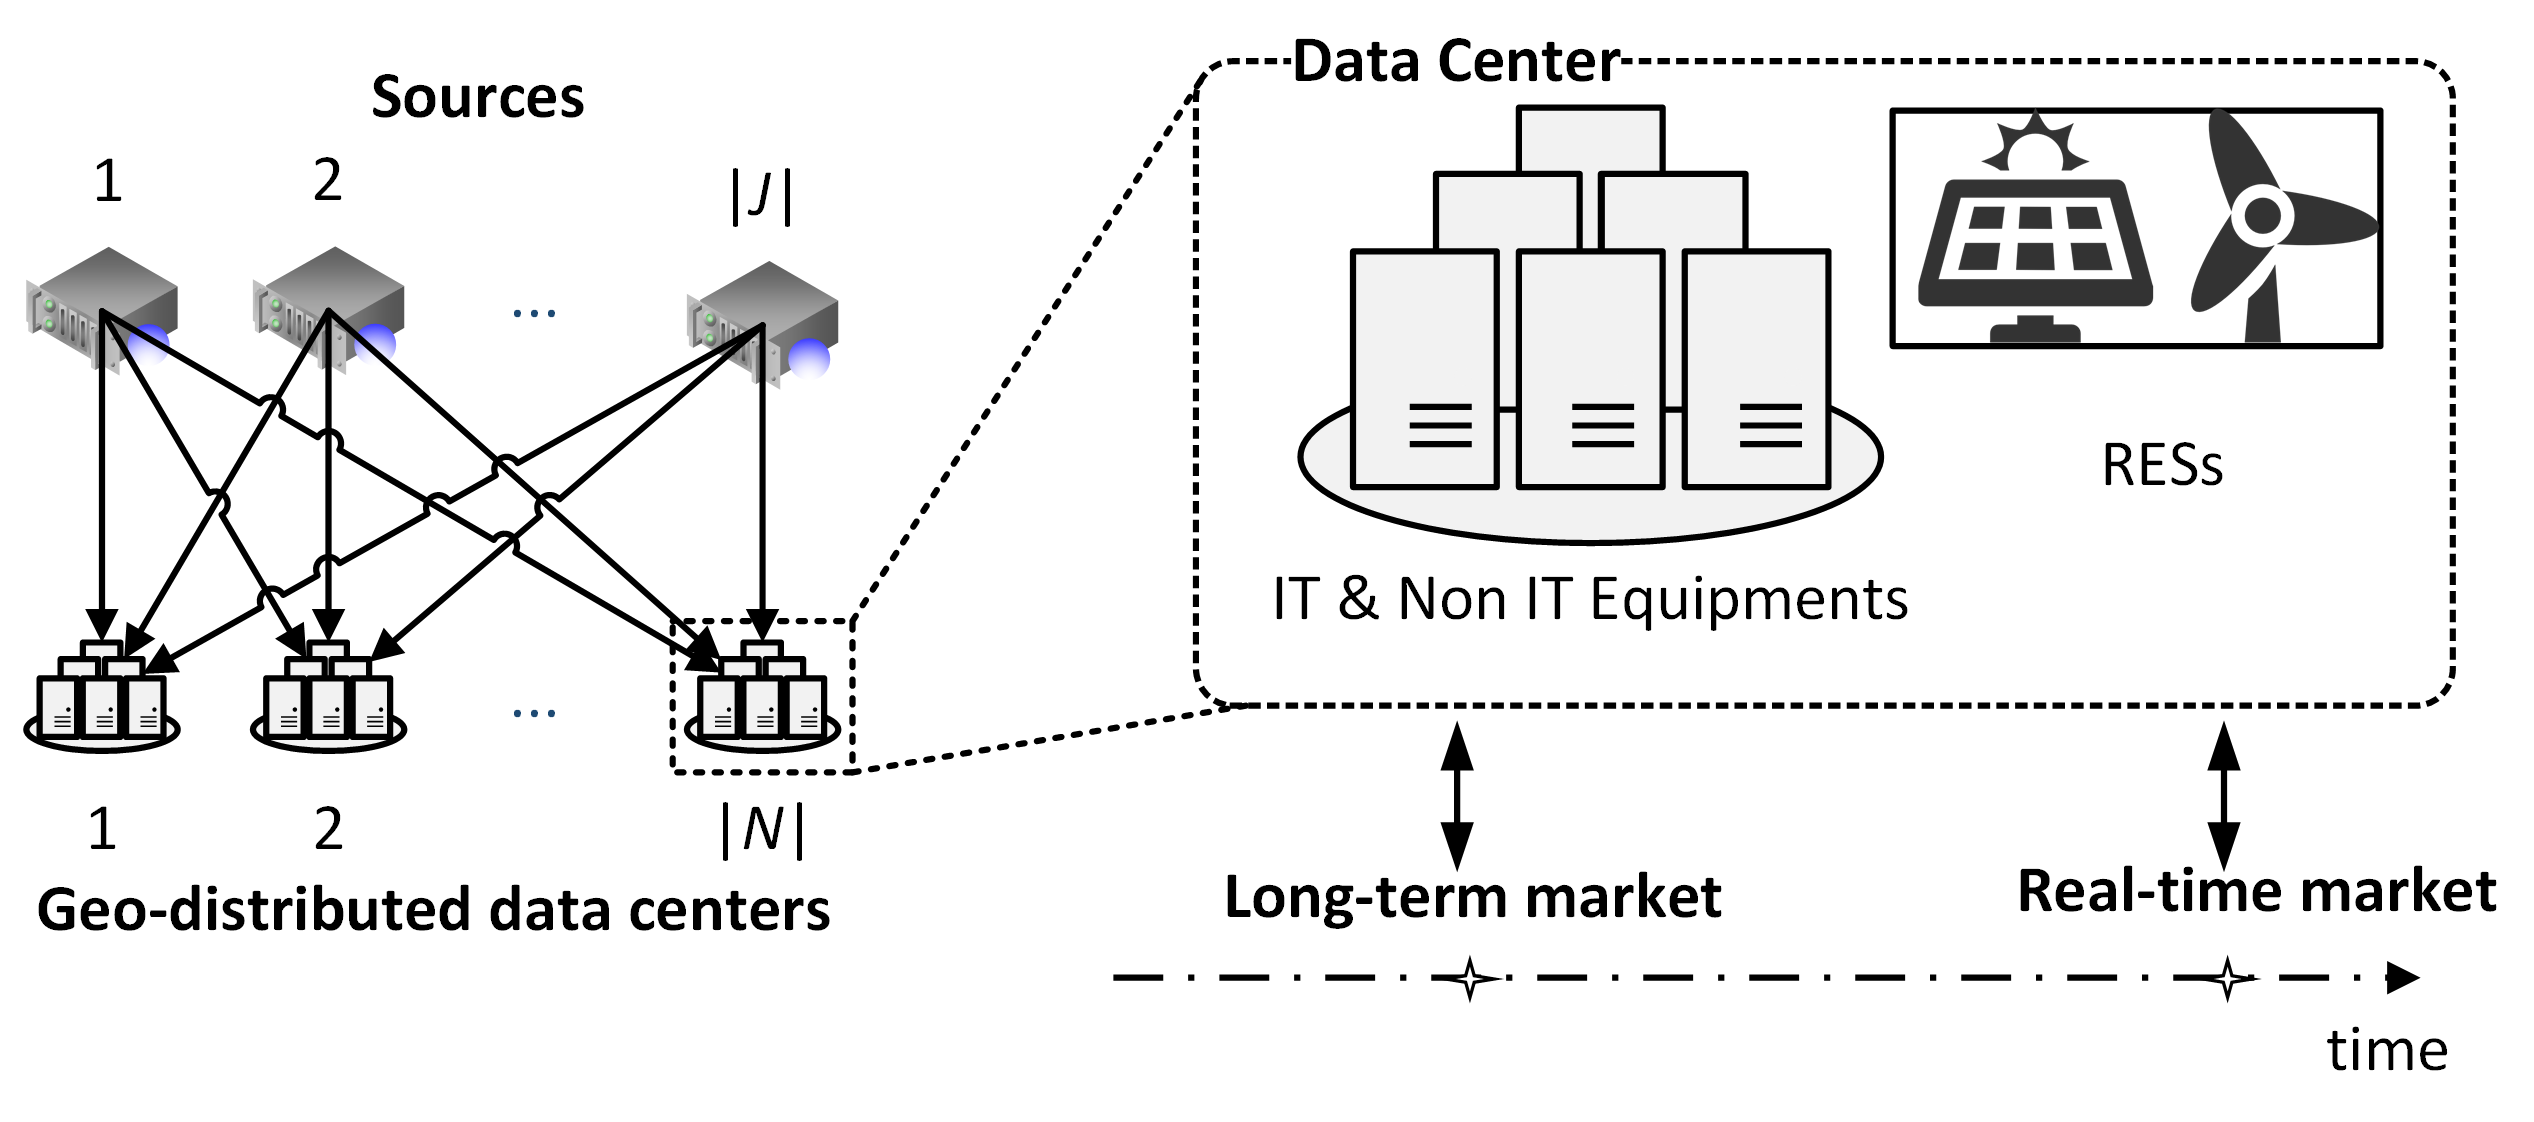
\includegraphics[width=1.0\linewidth]{figs/MultipleDataCenter}
%	\vspace{-0.8cm}
	\caption{Geo-distributed data centers in long-term and real-time markets.}
	\label{fig:MultipleDataCenter}
%	\vspace{-0.3cm}
\end{figure}

\textbf{Geo-distributed data centers.} We consider a set $N$ of geo-distributed data centers serving workload demands from a set $J$ of sources as illustrated in Figure \ref{fig:MultipleDataCenter}. The workload demand from each source is split between the $|N|$ data centers. Here, a source can represent the aggregate demand from a group of local users, such as users of a particular city, ISP, or geographical region. Each data center has access to renewable energy sources. Further, each data center participates in a (local) long-term electricity market and a (local) real-time electricity market. In other words, each data center $i$ can buy electricity ahead of time in its long-term market, and can also buy additional electricity in its real-time market if necessary. %Note that different data centers may buy from different markets that are locally available to them.

\textbf{Energy procurement system (EPS)}. Our proposed energy
procurement system for geo-distributed data centers is depicted in
Figure \ref{fig:SystemArchitecture}. There are three main components,
namely, the long-term forecaster, the energy procurement
(EP) in long-term markets and the geographical load balancing (GLB). The long-term forecaster provides the forecasted
information for the energy procurement. The forecasted information
includes the predicted values and the prediction error distributions
of IT workload, renewable energy generations, and electricity
prices. We design the algorithms for the long-term forecaster in
Section \ref{sec:dataAnalysis}. The EP component procures electricity
for each data center in the corresponding long-term markets (at time
$t = -T_l$) based on the electricity prices in the long-term markets
and \emph{forecasts} of real-time prices, workload, and renewable
generation. The GLB component (at time $t = 0$) distributes (routes)
the realized workload from sources to data centers, provisions the
required computing capacity at each data center, and procures
additional electricity as needed in the real-time markets.

\textbf{Data center}. Let $M_i$ denote the number of servers in data
center $i$. The number of active servers at real-time (time $t=0$) is
denoted by $m_i,$ which is a control parameter. In practice, there can
be more than a hundred thousand servers in a single data center. Thus,
in our mathematical modeling, we treat $m_i$ as a real number
satisfying $0 \leq m_i \leq M_i.$

\begin{figure}[!t]
	\centering
	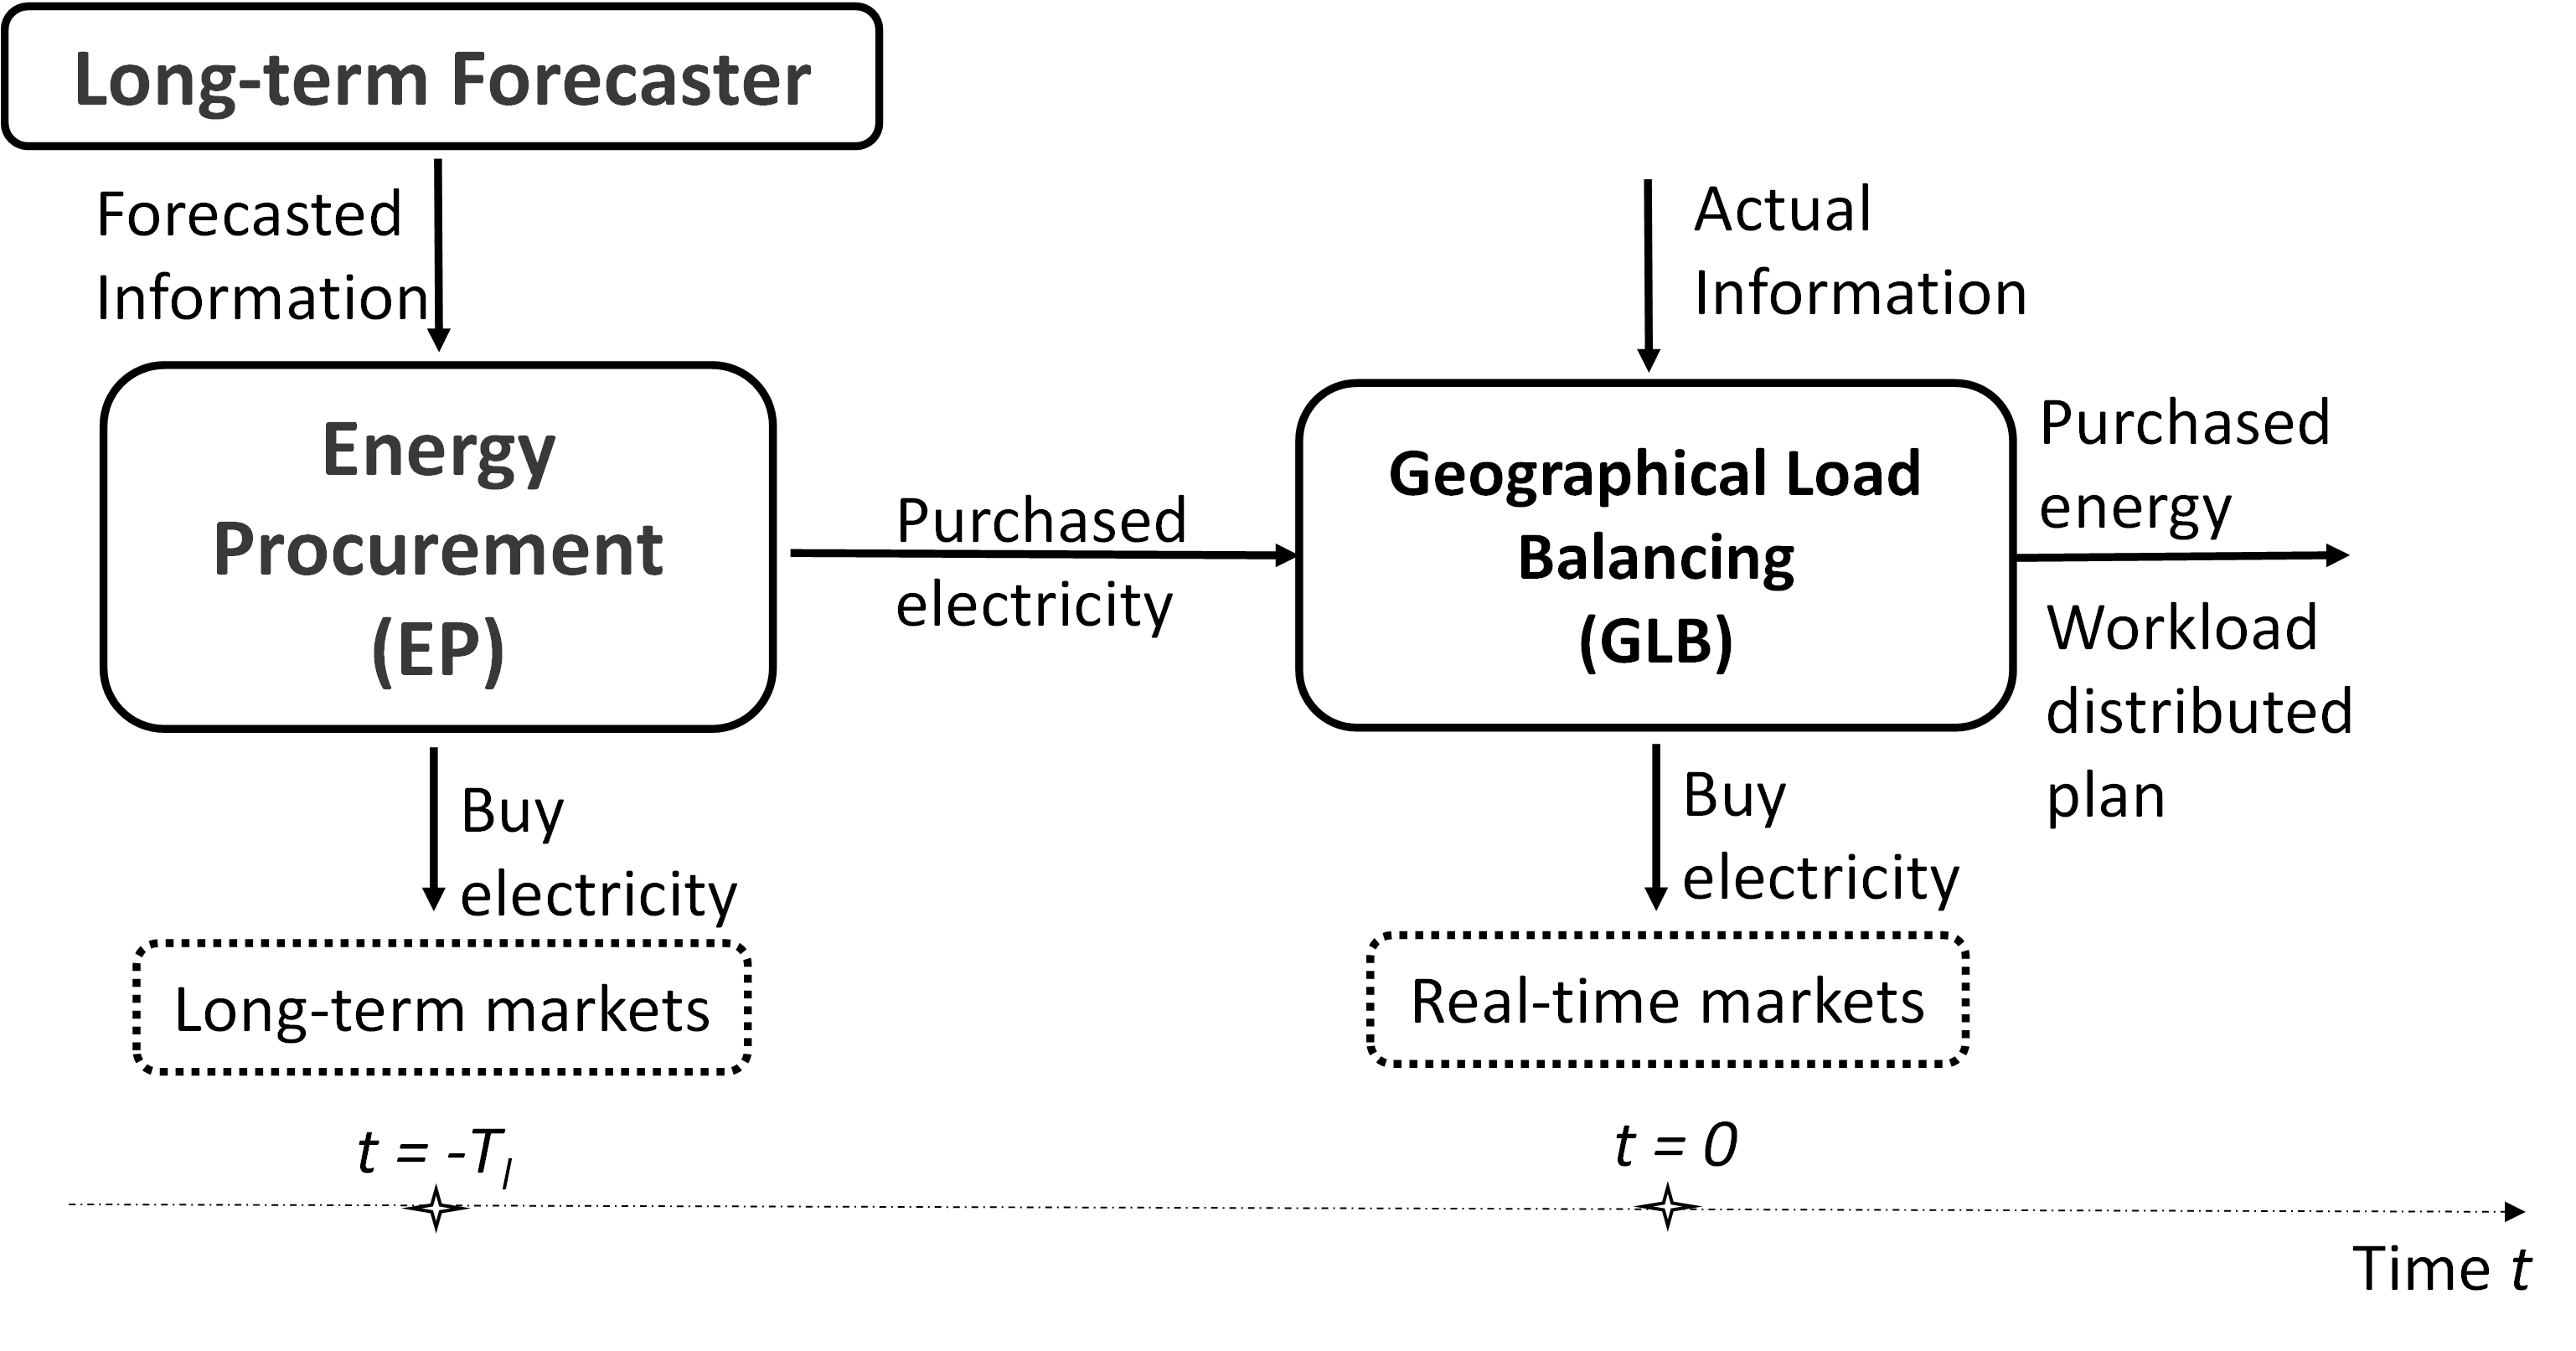
\includegraphics[width=1.0\linewidth]{figs/SystemArchitecture}
%	\vspace{-0.8cm}
	\caption{Energy Procurement System (EPS) Architecture for geo-distributed data centers.}
	\label{fig:SystemArchitecture}
%	\vspace{-0.3cm}
\end{figure}

At time $t = 0,$ the power consumption of data center $i$ is denoted
by $d^r_i.$ In general, the power consumption of data center $i$ is
dependent on the number of active servers $m_i$ and the workload
arrival
$\lambda_i$. %Let $d^r_i = O_i(m_i, \lambda_i),$ where the power consumption function $O_i(\cdot)$ is non-decreasing in $m_i$ and $\lambda_i$.
For simplicity, we assume that $d^r_i = m_i$, which implies that the
power consumption is proportional to the number of active servers, and
is independent of the workload $\lambda_i$.\footnote{The
  proportionality constant relating the number of active servers and
  the power consumption is taken to be 1 without loss of
  generality. %Also, our analysis can be easily generalised to the case
  % $d^r_i = O_i(m_i, \lambda_i),$ where the function $O_i$ is
  % continuously differentiable, convex, and non-decreasing in each
  % coordinate.
} %This model is can be applied to other cases, such as
               %the linear power consumption model
               %\cite{rao2011hedging,liu2011greening,
               %liu2012renewable}.


\textbf{Workload}. Workload demand from source $j$ in real-time ($t = 0$) is denoted as $L^r_j.$ We assume that the exact realization of the random vector $\Vector{L}^r = (L^r_j,j \in J)$ is known to the cloud provider at time $t = 0,$ and is an input to GLB. Let $\lambda_{ij}$ denote the distributed workload arrival from source~$j$ to data center $i$ at time $t = 0$ (set by GLB). Thus,
\begin{eqnarray*}
	\label{eq:constraintWorkload1}
	L^r_j = \sum_{i\in N}^{}\lambda_{ij}  & \quad (j\in J), \\
	\label{eq:constraintWorkload2}
	\lambda_i = \sum_{j\in J}^{}\lambda_{ij} & \quad (i \in N).
\end{eqnarray*}
Here, $\lambda_i$ denotes the aggregate workload routed to data center $i.$

\textbf{Renewable energy}. Data centers can utilize their integrated RESs. Let $w^r_i$ denote the renewable energy generation at data center $i$ in real-time ($t=0$). We assume that the exact realization of the random vector $\Vector{w}^r = (w^r_i,i \in N)$ is known at time $t = 0,$ and is an input to GLB. 
%Moreover, we assume that $w^r_i$ is a continuous random variable for each $i \in N.$

%\david{use "at time $t=0$" or "in real-time ($t=0$)"}

\textbf{Electricity price}. For each data center, the cloud provider can purchase electricity at time $t=-T_l$ in the local long-term market and then purchase any additional electricity needed in the local real-time market at time $t = 0.$ For data center~$i,$ let $p^{l}_i$ denote the long-term price for 1 unit of electricity, and $p^{r}_i$ denote the real-time price for 1 unit of electricity. We assume that $\Vector{p}^l = (p^l_i,i \in N)$ is fixed (or equivalently, is known at the time of the long-term procurement), and $\Vector{p}^r= (p^r_i, i \in N)$ is a random vector whose exact value is known is known at time $t = 0$ and is an input to GLB.

Note that the real-time workload $\Vector{L}^r,$ the real-time
renewable generation $\Vector{w}^r,$ and the real-time electricity
prices $\Vector{p}^r$ are unknown at the time of the long-term
procurement by the EP component, but are known at the time of
operation of the GLB component. We assume that the random vector
$(\Vector{L}^r,\Vector{w}^r,\Vector{p}^r)$ is jointly continuous. In
addition, all the $w^r_i$, $L^r_j$, and $p^r_i$ are assumed to be
bounded random variables.
% $\Exp{w^r_i} < \infty ,\Exp{p^r_i} < \infty$ and $\Exp{L^r_j} < \infty$.

% From the point of view of long-term markets, all the variables in
% real-time are random variables. Hence, workload $L^r_j$, renewable
% energy generation $w^r_i$, and electricity price $p^r_i$ are the
% random variables at time $t=-T_l$. Naturally, they are bounded by
% finite numbers.

\subsection{Cost model}

The total cost of operating geo-distributed data centers in composed of a delay cost and an energy cost. The delay cost is the monetary cost incurred due to the delay in processing the arriving workload. The energy cost is the total electricity bill from the long-term and real-time markets.

%\new{
\textbf{Delay cost}. We consider both the network delay between data centers and sources and the processing time within a data center. The network delay $\pi_{ij}$ captures the delay that propagates the workload $\lambda_{ij}$ from source $j$ to data center $i$. The queuing delay  $g_i(m_i,\lambda_i)$ denotes the delay at data center $i$ to process its arrival workload $\lambda_i$. %We assume that $g_i$ is strictly decreasing
%in $m_i$, strictly increasing in $\lambda_i$, and jointly convex in both
%$m_i$ and $\lambda_i$.
For stability, we need that $\lambda_i < m_i \mu _i$.
Here, $\mu _i$ is the service rate of a server in data center $i$.
Thus, we define $g_{i}(m_i, \lambda_{i}) = \infty$ for $\lambda_i \geq m_i \mu_i.$
%}

%\new{
We model the delay cost $h_{ij}(m_i,\lambda_i)$ of routing and processing each unit of workload from source $j$ to data center $i$ as follows.
%}
\begin{eqnarray}
\label{eq:gen_delaycost}  
h_{ij}(m_i, \lambda_{i}) = \beta \big ( g_i(m_i,\lambda_i) + \pi_{ij}  \big ).
\end{eqnarray}
%\new{
Here, the parameter $\beta$ weighs the delay relative to the energy
cost. While {\eqref{eq:gen_delaycost}} assumes a linear relationship
between incurred delay and the associated monetary cost (as is
suggested in {\cite{Beheshti2012PerformanceImpact}}), our model allows
for a non-linear (convex) relationship between delay and its monetary
cost to the cloud provider. The delay cost of transmitting workload
{$\lambda_{ij}$} from source $j$ to data center {$i$} is computed as
$\lambda_{ij}h_{ij}(m_i,\lambda_i)$.  We assume that
$h_{i,j}(m_i, \lambda_{i})$ is continously differentiable over
$0 \leq \lambda_i < m_i \mu_i,$ and that
$\lambda_{ij}h_{ij}(m_i, \lambda_{i})$ is jointly convex with respect
to $m_i$ and $\lambda_{i}.$
%}


A specific instance of the delay cost function $h_{ij}$ that satisfies
the above assumptions, and which we use in our experimental
evaluations, is
\begin{eqnarray}
\label{eq:delaycost}
%h_{ij}(m_i, \lambda_{i}) = \beta \bigg (\frac{1}{\mu_i - \lambda_i/m_i} + \pi_{ij}  \bigg ) & \quad (\lambda_i < m_i \mu_i),
h_{ij}(m_i, \lambda_{i}) = \beta \bigg (\frac{1}{\mu_i - \lambda_i/m_i} + \pi_{ij}  \bigg ) & \quad (\lambda_i < m_i\mu_i),
\end{eqnarray}
%\new{
where the first term $\frac{1}{\mu_i - \lambda_i/m_i}$ above
captures queuing delay at delay center $i,$ which is based on the
well-known mean delay formula for the M/GI/1 processor sharing
queue.
%} 

%%JK -- I don't think this generalization is correct.

%%be proportional to a certain range of delay
%\cite{Beheshti2012PerformanceImpact}.

%Here, $\mu_i$ is the service rate of servers in data
%center $i.$ We require that
%\begin{eqnarray*}
%	\lambda_i \leq m_i \mu_i & \quad (i\in N).
%\end{eqnarray*}


% There could be several ways to model the delay cost based on the
% responsive time. For instance, the lost revenue can be proportional
% to a certain range of delay \cite{Beheshti2012PerformanceImpact}. We
% assume that the delay cost of routing and processing each unit of
% the workload from source $j$ to data center $i,$ denoted
% $h_{ij}(m_i, \lambda_{i}),$ is jointly convex over $(m_i,
% \lambda_{i}).$



% Thus, we model the delay cost $h_{ij}(m_i, \lambda_{i})$ of routing
% and processing each unit of the workload from source $j$ to data
% center $i$ as follows.  We consider delay $h_{ij}(m_i, \lambda_{i})$
% in real-time when routing and processing each unit of workload from
% sources $j$ to data center $i$. We assume that $h_{ij}(m_i,
% \lambda_{i})$ is convex, increasing in $m_i$, and decreasing in
% $\lambda_{i}$. In particular, we use the following delay cost model
% for further analysis and evaluation.

%$p^r_i$ has to be in an acceptable range $ [\underbar{p}^{r},\bar{p^{r}}] $. Let $f_{p^{r}}(\cdot)$ is the probability density function of the real-time prices. $f_{p^{r}}(\cdot)$ is assumed to be continuous over $ (\underbar{p}^{r},\bar{p^{r}}) $.

\desc{Energy cost}

\textbf{Energy cost}. Let $q^l_i$ and ${q}_i^r$ respectively denote the amount of electricity purchased in the long-term market and the real-time market by data center $i.$ Here, we require that sufficient electricity is procured to process the workload routed to each data center as $$q^r_i + w^r_i + q^l_i \geq d^r_i = m_i \quad (i \in
N).$$
%The the amount of long-term energy $q^l_i$ and the amount of real-time energy $q^r_i$ are related as
%\begin{align}
%q^r_i &= [m_i - w^r_i - q^l_i]_+,
%\end{align}
%where $[x]_+$ is equal to the maximum of $\{x,0\}$. Hence, $q^r_i \geq 0$ and $q^r_i \geq  m_i - w^r_i - q^l_i$.
%JK -- I think these deductions should come later.
The electricity bills of data center $i$ in the long-term market and the real-time market are respectively computed as
\begin{align*}
R^l_i(q^l_i) &= p^l_i q^l_i & i\in N, \\
R^r_i(q^r_i) &= {p}_i^r q^r_i & i \in N.
\end{align*}
%where $R^l_i(q^l_i)$ is the long-term electricity cost and $R^r_i(q^r_i)$ is the real-time electricity cost.

% \begin{eqnarray}
% \label{eq:totalCost}
% F(\Vector{q}^l,\Vector{m}, \Vector{\lambda}, \Vector{p}^r) = \sum_{i\in N}^{} R^l_i(q^l_i) + F^r(\Vector{q}^l,\Vector{p}^r,\Vector{L}^r,\Vector{w}^r)
% \end{eqnarray}
% where $\Vector{q}^l,\Vector{m},$, $\Vector{\lambda}$, and $\Vector{p}^r$ are the vectors of $\{q^l_i\}_{i \in N}, \{m_i\}_{i \in N},$, $\{\lambda_{ij}\}_{i \in N, j \in J}$, and $\{p^r_i\}_{i\in N}$ respectively. The real-time cost objective computed as
% \begin{equation}
% \label{eq:rt-obj2}
% F^r(\Vector{q}^l,\Vector{p}^r,\Vector{L}^r,\Vector{w}^r) =  \sum_{i \in N}^{} R_i^r(q^r_i)+ \beta\sum_{i,j \in N,J} \lambda_{ij}h_{ij}(m_i,\lambda_i),
% \end{equation}
% where $\beta$ weighs the importance of the delay cost.

% We notice that working out the total cost \eqref{eq:totalCost} is extremely challenging because there are bidirectional influence between two different time-scales, i.e., long term and real-time. In chronological order, our energy procurement system first computes the best long-term procurement, $\Vector{q}^l$. However, the system has to consider its impact on real-time markets which are very uncertain and vise versa. It is because our energy procurement system also minimizes the total cost $F^r(\Vector{q}^l,\Vector{m},\boldsymbol{\lambda} , \Vector{p}^r, \Vector{w}^r)$ in real-time, denoted as 
% $$\min_{} F^r(\Vector{q}^l,\Vector{m},\Vector{\lambda},\Vector{p}^r,\Vector{w}^r).$$



% %\subsection{Geo-graphical load balancing at real-time}

\subsection{Formulation of optimal energy procurement in multi-timescale markets}

In this section, we describe the optimization formulation for optimal energy procurement. Recall that the total cost of operating geo-distributed data centers in our two-timescale market setting is the sum of the energy cost and the delay cost, given by $$F = \sum_{i\in N}^{} R^l_i(q^l_i) + \sum_{i \in N}^{} R_i^r(q^r_i)+ \sum_{i \in N,j \in J} \lambda_{ij}h_{ij}(m_i,\lambda_i).$$
We seek to minimize $\Exp{F}$ subject to the aforementioned constraints. Note that this optimization is performed on two timescales, with different sets of information available at each. The EP component optimizes the long-term procurements $\Vector{q}^l = (q^l_i, i\in N)$ given only distributional information of the real-time workload $\Vector{L}^r,$
the real-time renewable generation $\Vector{w}^r,$ and the real-time electricity prices $\Vector{p}^r.$ The GLB component optimizes the workload routing $\Vector{\lambda} = (\lambda_{ij},i\in N,j \in J),$ the number of active servers $\Vector{m} = (m_i,i \in N)$ at the data centers, and the real-time procurements $\Vector{q}^r = (q^r_i,i \in
N)$ given the prior long-term procurements $\Vector{q}^l,$ and the exact realization of $(\Vector{p}^r,\Vector{L}^r,\Vector{w}^r).$
Below, we first formalize the real-time optimization, followed by the long-term optimization.

\textbf{Geographical load balancing in real-time markets}. 

Note that in real-time, GLB optimizes the real-time procurements
$\Vector{q}^r$, the numbers of active servers $\Vector{m}$, and the workload routing $\Vector{\lambda},$ given the long-term procurements $\Vector{q}^l$ and the realization of the random vector $(\Vector{p}^r,\Vector{L}^r,\Vector{w}^r).$ The total cost as seen by GLB is $$F^r(\Vector{q}^r, \Vector{m},\Vector{\lambda},\Vector{p}^r)
:= \sum_{i \in N}^{} R_i^r(q^r_i)+ \sum_{i\in N, j \in J}
\lambda_{ij}h_{ij}(m_i,\lambda_i).$$ Thus, the real-time optimization is defined as follows.

\vspace{0.1in}
\begin{subequations}
	\begin{align}
	\text{\bf{GLB-RT}: } &  \min_{\Vector{m}, \Vector{\lambda}, \Vector{q}^r} F^r(\Vector{q}^r, \Vector{m},\Vector{\lambda},\Vector{p}^r) \nonumber \\
	\mbox{s.t. } \nonumber \\
	\label{eq:GLB-RT_c1}
	&\lambda_{ij} \geq 0  \quad \forall i \in N,j \in J \\
	&\sum_{i\in N}^{} \lambda_{ij} = L^r_j \quad \forall j \in J \\
	\label{eq:GLB-RT_c}
	% &\sum_{j\in J}^{} \lambda_{ij} = \lambda_i &\forall i \in N \\
	&\lambda_i \leq m_i \mu_i,   \quad \forall i \in N\\
	&0 \leq m_i \leq M_i \quad \forall i \in N \\
	\label{eq:GLB-RT_c2}
	&q^r_i \geq 0, \quad \forall i \in N \\
	\label{eq:GLB-RT_c3}
	& m_i - q^r_i - w^r_i \leq q^l_i \quad \forall i \in N
	\end{align}
\end{subequations}
\vspace{0.1in}

Since $p^r_i \geq 0,$ it easily follows that any solution of the above optimization problem satisfies $q^r_i =[m_i - w^r_i - q^l_i]_+,$ where $[x]_+ := \min\{0,x\}.$ Thus, the real-time objective can be re-written as 
\begin{equation}
\label{eq:rt-obj2}
\begin{array}{rl}
&\tilde{F}^r(\Vector{q}^l,\Vector{m},\Vector{\lambda},\Vector{p}^r,\Vector{w}^r) = \sum_{i \in N} p^r_i [m_i - w^r_i - q^l_i]_+ \\
& \qquad+ \sum_{i\in N, j \in J}
\lambda_{ij}h_{ij}(m_i,\lambda_i).    
\end{array}
\end{equation}
With this notation, GLB-RT can be equivalently expressed as follows.
\begin{subequations}
	\begin{align*}
	& \min_{\Vector{m}, \Vector{\lambda}} \tilde{F}^r(\Vector{q}^l,\Vector{m},\Vector{\lambda},\Vector{p}^r,\Vector{w}^r) \\
	\mbox{s.t. } \nonumber \\
	&(\Vector{m},\Vector{\lambda}) \in C(L^r).
	\end{align*}
\end{subequations}
Here, the convex compact set $C(L^r)$ is defined by the constraints
\eqref{eq:GLB-RT_c1}--\eqref{eq:GLB-RT_c2}.
%%to be moved to the appendix where this will be used.


GLB-RT problem is a convex optimization problem and hence can be solved efficiently using standard techniques \cite{boyd2004convex}. For instance, CVX (Matlab Software for Disciplined Convex Programming) tool \cite{grant2008cvx} can be used to solve GLB-RT. 
%In Section~\ref{sec:char_glb-rt}, we prove several interesting properties of the optimal solutions of GLB-RT.


\textbf{Energy procurement in long-term markets}. At time $t=-T_l$,
the cloud provider purchases electricity $\Vector{q}^l$ in
long-term markets that will be used at real-time. Note that
optimization of the long-term procurements has to be performed based
only on distributional information for the random vector
$(\Vector{p}^r,\Vector{L}^r,\Vector{w}^r),$ and subject to the
real-time optimization that will be subsequently performed based on
the realization of the random vector
$(\Vector{p}^r,\Vector{L}^r,\Vector{w}^r).$ 

Let us denote the optimal value of the optimization GLB-RT by
$F^{*r}(\Vector{q}^l,\Vector{p}^r, \Vector{L}^r, \Vector{w}^r).$ The
long-term objective is thus defined as $$F^l(\Vector{q}^l) :=
\sum_{i\in N} R^l_i(q^l_i) + \Exp{F^{*r}(\Vector{q}^l,\Vector{p}^r,
	\Vector{L}^r, \Vector{w}^r)}.$$ Note that the above expectation is
with respect to the random vector
$(\Vector{p}^r,\Vector{L}^r,\Vector{w}^r).$ The long-term optimization
problem is then given by:
\begin{subequations}
	\begin{align*}
	\text{\bf{EP-LT}: }  & \min F^l(\Vector{q}^l) \\
	\mbox{subject to } \nonumber \\
	& \Vector{q}^l \in \mathbb{R}^N_+.
	\end{align*}
\end{subequations}

The above optimization is more challenging than GLB-RT. In
Section~\ref{sec:char_ep-lt}, we prove that EP-LT is a convex
optimization and characterize the gradient of the objective
function. These results are then used to arrive at a provably optimal stochastic gradient algorithm in Section~\ref{sec:AlgorithmDesign}.
